\section{Using the application}

\subsection{Loading and viewing frames}

When you first load the model fitting application you will see a main window with four empty panes in the central area.

The very first step is to open a directory containing gait samples.
This can be done by selecting \emph{Open directory...} from the \emph{File} menu.

As shown in Figure \ref{manual:opendir} you should navigate to one of the \emph{gaitdata} directories on the DVD and click the \emph{Choose} button.
This will load the list of framesets (samples) in the upper left dock panel.
Clicking on one of these will load the list of frames into the second dock panel.

\begin{figure}[htb]
	\centering
	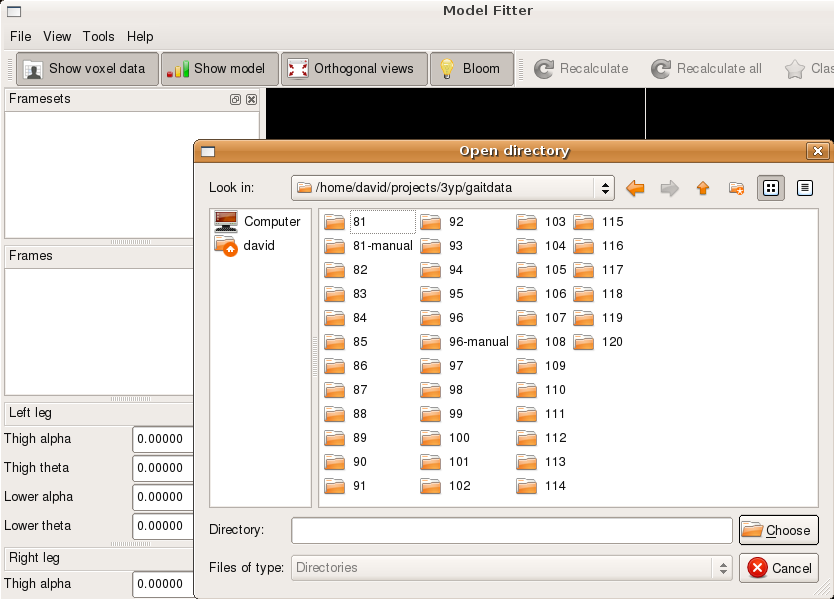
\includegraphics[width=8cm]{manual/opendir.png}
	\caption{Opening a directory containing gait samples.}
	\label{manual:opendir}
\end{figure}

The top-left, top-right and bottom-left views show front, side and overhead orthographic projections of the figure.
The bottom-right view shows a perspective projection.
This final view can be moved and rotated by the user with the following controls:

\begin{itemize}
	\item \textbf{Rotate} - click and drag inside the viewport.
	\item \textbf{Move} - hold the \emph{Shift} key, and click and drag inside the viewport.
\end{itemize}

The three orthographic projections can be toggled on and off by pressing the \emph{Orthogonal views} toolbar button.


\subsection{Model fitting and graph plotting}

Once you have selected a frame in the left dock panel you can start the modelfitting process by clicking the \emph{Recalculate} button on the toolbar.
This will open a progress dialog similar to the one shown in Figure \ref{manual:modelfitting}.

\begin{figure}[htb]
	\centering
	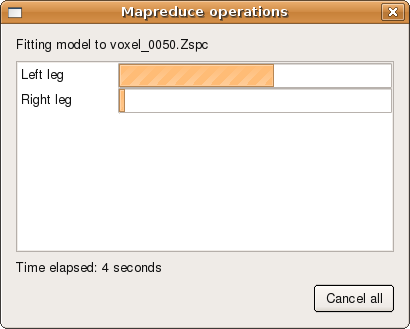
\includegraphics[width=6cm]{manual/modelfitting.png}
	\caption{Dialog displaying the progress of modelfitting operations.}
	\label{manual:modelfitting}
\end{figure}

The \emph{Recalculate All} button will run the modelfitting process on all the frames in the currently selected frameset.
Note that you can also process frames in bulk using the command line interface.
This is described in more detail in Section \ref{manual:commandline}

\bigskip
\noindent Several graph plotting facilities are available in the \emph{Tools} menu.
These all require the gnuplot utility to be installed and available in the system \$PATH.

\begin{itemize}
	\item \textbf{Plot energy graphs}.
		Only available immediately after the modelfitting process has completed.
		The data that is plotted is held in memory and not saved to disk, so it is discarded when opening another frame.
	\item \textbf{Plot params over time}.
		Plots the changes in the values of the various parameters over each of the frames in the frameset.
		Only frames that have previously had their model information calculated will be displayed in the graph.
		Figure \ref{manual:plotter} shows the graph plotting dialog.
	\item \textbf{Plot FFT graphs}.
		Runs a DFT on the data and displays the results.
		Magnitude and phase can be plotted individually, as well as the phase-weighted magnitude.
\end{itemize}

\begin{figure}[htb]
	\centering
	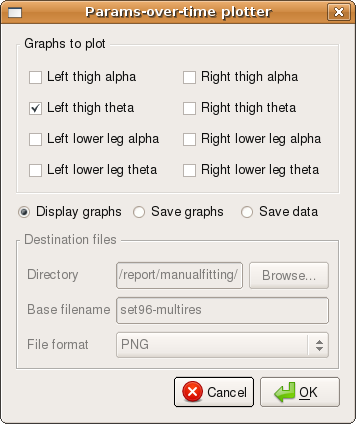
\includegraphics[width=6cm]{manual/plotter.png}
	\caption{A typical graph plotter dialog.}
	\label{manual:plotter}
\end{figure}

All graph dialogs have the option to display the graph, save the graph, or save the data that would be used to generate the graph.
The final option can be helpful if you need to use gnuplot manually to plot the data in different ways.


\subsection{Classification}

When you have calculated the model fitting for all frames in a frameset, you can click the \emph{Classify this Person} toolbar button to open the classification dialog.
When classifying a sample for the first time, the dialog will enter its signature into a database and use display it in a list for future classifications.
It will also display the ``distance'' from the sample you are classifying to all the other samples in the database.
This is a metric that determines the similarity between samples.

In Figure \ref{manual:classify} we can see that the sample being classified has a very similar gait to Sample 1 who was classified earlier.

\begin{figure}[htb]
	\centering
	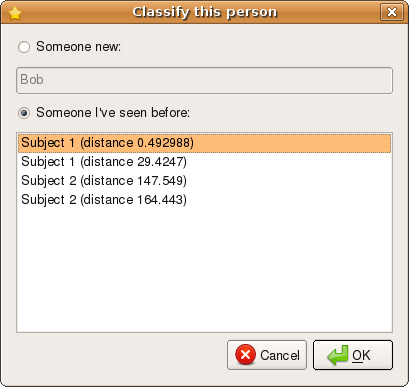
\includegraphics[width=6cm]{manual/classify.png}
	\caption{The classification dialog.}
	\label{manual:classify}
\end{figure}

Note that currently it is not possible to remove classifications from the database.
To do this you must edit the configuration directly:

\begin{itemize}
	\item \verb+~/.config/ECS/Modelfitting.conf+ on Unix
	\item \verb+~/Library/Preferences/uk.ac.soton.ecs.Modelfitting.plist+ on Mac OS X
	\item \verb+HKEY_CURRENT_USER\Software\ECS\Modelfitting+ on Windows
\end{itemize}



\section{Command line interface}
\label{manual:commandline}

It is possible to use the commandline interface to perform batch processing of frames on headless servers.

Note that sadly due to a bug in Qt it is not possible to use the command line interface on Unix without first applying a patch to the Qt sources.
The patch is provided on the DVD.
An issue has been raised with Trolltech and can be tracked by issue number 207245:

\verb+http://trolltech.com/developer/task-tracker+

\bigskip
\noindent A list of directories can be provided as commandline arguments to the modelfitting executable.
These will be processed sequentially:

\clearpage
\begin{lstlisting}[firstnumber=1,language=sh,frame=single]
$ ./modelfitting ../../gaitdata/81
Queueing all files in directory: ../../gaitdata/81
../../gaitdata/81/voxel_0058.Zspc: Starting...
../../gaitdata/81/voxel_0058.Zspc: Left leg finished

...
\end{lstlisting}

By default the thread pool creates one thread for every processor core in the system.
If one leg finishes processing before the other, one of these threads will sit idle and wait for the other leg to complete.
You can use the -j argument to specify the number of frames to process concurrently.
It is recommended to set this to 2 so that all the cores in the system will be working at any time.

\begin{lstlisting}[firstnumber=1,language=sh,frame=single]
$ ./modelfitting ../../gaitdata/81 -j 2
Queueing all files in directory: ../../gaitdata/81
../../gaitdata/81/voxel_0058.Zspc: Starting...
../../gaitdata/81/voxel_0059.Zspc: Starting...

...
\end{lstlisting}
